 \begin{center}
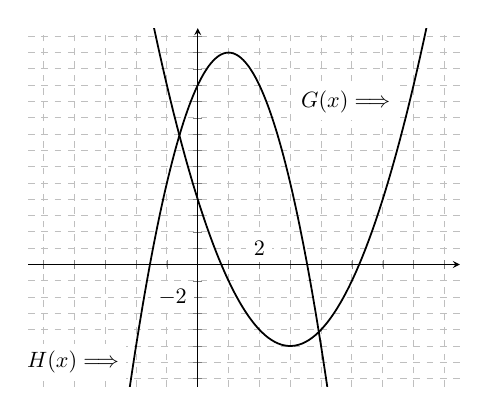
\begin{tikzpicture}[scale=0.8]\begin{axis}[axis lines=center,grid=both,grid style={dashed, gray!50!white}, xmin=-5.5,xmax=8.5,ymin=-7.5,ymax=14.5, xtick={-5,-4,...,8},xticklabel=\empty, ytick={-9,-8,...,14},yticklabel=\empty,]
\addplot[thick,samples=51,smooth,domain=-3:8]{(x-3)^2-5};
\addplot[thick,samples=51,smooth,domain=-3:5]{-2*x^2+4*x+11};
\draw(axis cs:2,0.1)node[anchor=south, rectangle, fill=white]{$2$};
\draw(axis cs:-0.1,-2)node[anchor=east, rectangle, fill=white]{$-2$};
\draw(axis cs:6.5,10)node[anchor=east,rectangle,fill=white]{$G(x)\Longrightarrow$};
\draw(axis cs:-2.3,-6)node[anchor=east,rectangle,fill=white]{$H(x)\Longrightarrow$};

\end{axis}
\end{tikzpicture}\end{center}
Graphs of the functions $G(x)$ and $H(x)$ are shown in the $xy$-plane above.  For which of the following values of $x$ does $G(x)+H(x)=0$?\\\\


\ifsat
	\begin{enumerate}[label=\Alph*)]
		\item $4 $ 
		\item $3 $ % 
		\item $2 $ 
		\item $1 $
	\end{enumerate}
\else
\fi

\ifacteven
	\begin{enumerate}[label=\textbf{\Alph*.},itemsep=\fill,align=left]
		\setcounter{enumii}{5}
		\item $4 $ 
		\item $3 $ % 
		\item $2 $ 
		\addtocounter{enumii}{1}
		\item $1 $
		\item None of these. 
	\end{enumerate}
\else
\fi

\ifactodd
	\begin{enumerate}[label=\textbf{\Alph*.},itemsep=\fill,align=left]
		\item $4 $ 
		\item $3 $ % 
		\item $2 $ 
		\item $1 $
		\item None of these. 
	\end{enumerate}
\else
\fi

\ifgridin
 $3 $ % 
		
\else
\fi

